\section{METHODOLOGY}
\label{sec:METHODOLOGY}

\subsection{Manipulating Figures}

\autoref{fig:flow-chart} is an example of adjusting the figure to only 50\% of the page width and formatting it in center-alignment.

    \begin{figure}[ht]
        \caption{System Flow Chart of Object Recognition with Voice Feedback}
        \centering
        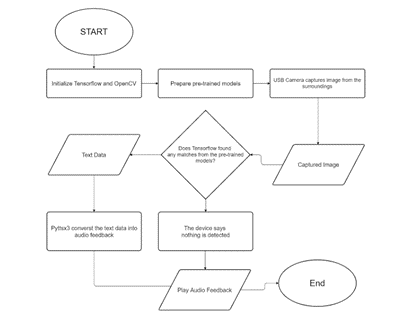
\includegraphics[width=0.5\textwidth]{Images/system-flow-chart.png}
        \label{fig:flow-chart}
    \end{figure}

\subsection{Manipulating Figures}

Meanwhile \autoref{fig:power-circuit} is an example of adjusting the figure to 80\% of the page width and formatting it right-aligned using \verb|\raggedleft|.

    \begin{figure}[ht]
        \caption{Power Supply Circuit}
        \raggedleft
        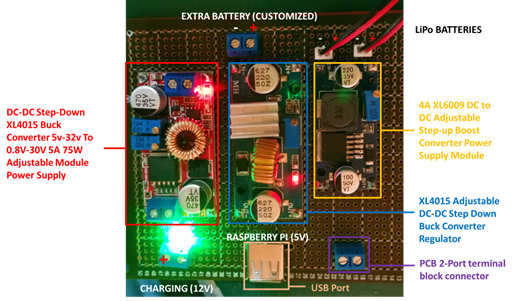
\includegraphics[width=0.8\textwidth]{Images/power-supply-circuit.png}
        \label{fig:power-circuit}
    \end{figure}